\documentclass[a4paper]{article}

\usepackage[english]{babel}
\usepackage[utf8]{inputenc}
\usepackage{amsmath}
\usepackage{graphicx}
\usepackage{cite}
\usepackage{pgfplots}   % pacote para uso do pgfplots

\title{Hand Tracking Using Distinct OpenCV Methods and Analysis of their Accuracy}

\author{Francisco Jose Nardi Filho, 163129\\ Lucas Gasparetto Farris, 103147}

\date{June 24, 2015}

\begin{document}
\maketitle

\begin{abstract}
\noindent
Mean Shift, Camshift and KLT are three successful approaches to visual tracking. However, each of them have their particular strengths and weaknesses. In this paper, we intend to present implementations of each distinct method from the OpenCV library and make an accuracy and  performance analysis for a hand tracking case. Fifteen videos taken from YouTube showing diverse situations as teaching of the American signal language alphabet, Mudras (gestures from an Indian dance), as well as guitar playing  were used as dataset to run the algorithms and perform the hand tracking. The hand position on these one-minute videos was manually annotated prior to the methods' accuracy and performance analysis. Extensive experimental results demonstrate that KLT outperforms Mean shift and Camshift regarding accuracy score, while Camshift outperforms Mean shift and KLT regarding accuracy hits, in hand tracking considering the provided database. Our approach produces reasonable tracking while handling regularly rapid motion. All the codes and videos can be found at https://github.com/luksfarris/VideoTrackingMO446. 
\end{abstract}

\section{Introduction}
Object tracking is to determine the position of the object at each frame of a video sequence. Reliable visual tracking is indispensable in several fields such as: ambient intelligent systems, augmented reality, human–computer interaction, video compression, and robotics. However, the task of robust tracking is very challenging regarding fast motion, occlusion, structural deformation, illumination variation, background clutters, and real-time restriction. Tracking algorithms can be divided into two categories.
\par
The first category is deterministic method. Mean-Shift  is a typical example. This method finds the local maximum of probability distribution in the direction of gradient. It is usually more accurate and quick in tracking than the probabilistic multi-hypothesis tracking algorithm. But it may run into trouble when similar objects are presented in background or when complete occlusion occurs. Camshift is called the Continuously Adaptive Mean Shift algorithm which is a modified algorithm of Mean-Shift.
\par
The second category is probabilistic method. The representative method is particle filter which is a multi-hypothesis tracking algorithm under the Bayesian framework . Due to particle filter’s non-Gaussian non-linear assumption and multiple hypothesis property, they have been successfully applied to visual tracking, and show unique merit in cluttered environment. However, the inefficiency in sampling (due to the problem of degeneracy and impoverishment) and the huge computational complexity limit the usefulness of particle filter in on-line tracking \cite{Yin2011}.
\par
Therefore, each method has its own advantages and disadvantages, manners to overcome the challenges described before. Aiming to find the optimal OpenCV method for hand tracking, and being aware of the nature of their categories, we have chosen four techniques very present in the literature of the state-of-art hand tracking, which are: Mean Shift, Camshift using SIFT keys, KLT and Particle Filtering.
\par
Videos extracted from YouTube having about 1 minute of duration and showing diverse situations as teaching of the American signal language alphabet, Mudras (gestures from an Indian dance), as well as guitar playing  were used as dataset to run the algorithms and perform the hand tracking. 
\par
A metric based on the matching between the annotated hand position on the videos and the hand position that was identified by the algorithm was defined in order to analyze the the algorithm's score and hits accuracy. While one considered how "close" the match happened, another just counted if there one some match or not. Extensive experimental results demonstrate that KLT outperforms Mean shift and Camshift regarding accuracy score, while Camshift outperforms Mean shift and KLT regarding accuracy hits, in hand tracking considering the provided database. Our approach produces reasonable tracking while handling regularly rapid motion.

\section{Related work}
There have been done many works in hand tracking. \cite{Kolsch2004} designed a fast tracking algorithm that combined Kanade-Lucas-Tomasi(KLT) flocks and k-nearest neighborhood. Based on the pros and cons of particle filter and mean shift, \cite{Shan2007} proposed a new algorithm, Mean Shift Embedded Particle Filter (MSEPF), in which mean shift is performed on each of the particles after they are propagated, so that the particles are "herded" to nearby local modes with large probability. Thus, the problem of degeneracy, where the weights of most particles become negligibly small after a few iterations, is tackled effectively. It is also claimed that as MSEPF can make better estimation of posterior even with a smaller set of samples, the computation cost is reduced proportionally. \cite{Maggio2005} also proposes a hybrid particle filtering and mean shift tracking algorithm, however using one more feature: an adaptive state transition model with updating variances. The update process is driven by the variability of the target in previous frames. 
\par
In another perspective, \cite{Ning2012} presents a scale and orientation adaptive mean shift tracking (SOAMST). It addresses the problem of how to estimate the scale and orientation changes of the target under the mean shift tracking framework. In the original mean shift tracking algorithm, the position of the target can be well estimated, while the scale and orientation changes can not be adaptively estimated. Considering that the weight image derived from the target model and the candidate model can represent the possibility that a pixel belongs to the target, it is shown that the original mean shift tracking algorithm can be derived using the zero th and the first order moments of the weight image.
\par
There are still some works as in \cite{Min1997}, which performs hand detection first extracting the images of hands (or palms) by mapping a circle plate in the candidate regions of hand and the center point of circle of same skin color. The mapping is done by employing Bresenham’s Midpoint circle scan-conversion algorithm for identification of the regions that cover the palm. As soon as the area matches the circle, it is added an initial position condition relative to the face to filter other noise regions before starting hand tracking. The hand detection method is applied on the fixed search window region for hand tracking. The boundary of hand is calculated and the centroid point of hand region is determined. Through iteration of hand tracking process, it is possible to obtain the motion trajectory of the hand so-called gesture path from connecting hand centroid points set.

\section{Experiments}
In this section, we carry out experiments to evaluate the accuracy of the developed hand tracking algorithms on 15 video sequences. The majority of the videos show a single hand most part of the time. However, there are many changes in the camera focus, which increases difficulty for the algorithms to keep track of the hand correctly. 
\par
Once the videos were annotated, the center of the hand in every frame, in every video is known. Therefore, the hand itself is represented by a circumference of fixed radius ($20 pixels$). In turn, the algorithms return a convex polygon with the region they understand as being the hand's most probable location. A grade is assigned to the algorithm's score. The grade consists of the following formula: 
\begin{itemize}
	\item $0$ if the annotated point is not inside the polygon.
    \item Otherwise $\dfrac{Annotated Area}{Polygon Area}$
\end{itemize}

\subsection{Mean Shift}
We used a straightforward approach, the algorithm is initialized with the video file path, and the coordinates of a region of interest (top left corner coordinates, width and height). For each frame, the histogram backprojected image of it was used. On each frame, the algorithm runs 10 iterations. The corners of each rectangle generated for each frame are saved. 


\begin{figure}[h]
\centering
\includegraphics[width=90mm]{mean.png}
\caption{Meanshift Polygon}
\end{figure}

\subsection{Continuously Adaptive Meanshift}
In this implementation we used the same parameters as the previous approach. CAMeanshift returns rotated rectangles, that can be represented in less parameters than all corners, but we chose to represent it as a list of all corners, to make the polygon evaluation tool generic.

\begin{figure}[ht!]
\centering
\includegraphics[width=90mm]{cam.png}
\caption{CAMeanshift Polygon}
\end{figure}

\subsection{Good Features To Track + Optical Flow}
On this approach we used OpenCV's Good Features To Track and KLT implementations. The specific parameters can be found in our code. We run the feature detector on a region of interest, and the detected points are observed throughout the video. We calculate the convex hull of the points, and save the resulting convex polygon. On each new frame, points may move, and the process restarts.

\begin{figure}[ht!]
\centering
\includegraphics[width=90mm]{klt.png}
\caption{KLT Polygon}
\end{figure}

\subsection{Evaluation}
After running the previous algorithms, the evaluation script reads all the polygons and the annotations, calculates the mean of the score of each algorithm, in each frame. We also calculate the total number of times each algorithm generated a polygon that contained the reference point.


\section{Results and discussion}

In Tables and Plots \ref{tabela1} and \ref{tabela2}, the results of each video in the dataset can be found.

\begin{table}[h]
\centering
\caption{Score}
\label{tabela1}
\begin{tabular}{|l|l|l|l|l}
\cline{1-4}
Index  & MS   & CAMS    & KLT &  \\ \cline{1-4}
1  & 0.017868877787106992   & 0.04834071999572289    & 0.048682322332621514 &  \\ \cline{1-4}
2  & 0.20464166745283086    & 0.033533440492696666   & 0.279069074174562    &  \\ \cline{1-4}
3  & 0.22439947525641354    & 0.093966703525928355   & 0.13620796357320028  &  \\ \cline{1-4}
4  & 0.016505083791994116   & 0.0060377125773232983  & 0.057772637930407995 &  \\ \cline{1-4}
5  & 0.099859793584633982   & 0.005193923207979797   & 0.0                  &  \\ \cline{1-4}
6  & 0.1901238237004759     & 0.0087698955142402266  & 0.13834897983806818  &  \\ \cline{1-4}
7  & 0.00051611056428611194 & 0.00037596389411216494 & 0.03549622940056314  &  \\ \cline{1-4}
8  & 0.042727525919647236   & 0.024013642802500183   & 0.11253166528744955  &  \\ \cline{1-4}
9  & 0.0026490253174241774  & 0.015121985308645959   & 0.17669007018779948  &  \\ \cline{1-4}
10 & 0.0                    & 0.020418527632106147   & 0.2250952493848905   &  \\ \cline{1-4}
11 & 0.0013612595837281677  & 0.0093192832530630734  & 0.2713289912518628   &  \\ \cline{1-4}
12 & 0.023374945339209762   & 0.035467315820262267   & 0.2325098760543383   &  \\ \cline{1-4}
13 & 0.0                    & 0.018246176158849603   & 0.02160098085837417  &  \\ \cline{1-4}
14 & 0.12659454841132223    & 0.046426220629364294   & 0.4013802649180197   &  \\ \cline{1-4}
15 & 0.010924003231906974   & 0.00020932749656048277 & 0.0                  &  \\ \cline{1-4}
\end{tabular}
\end{table}

\begin{figure}
\centering
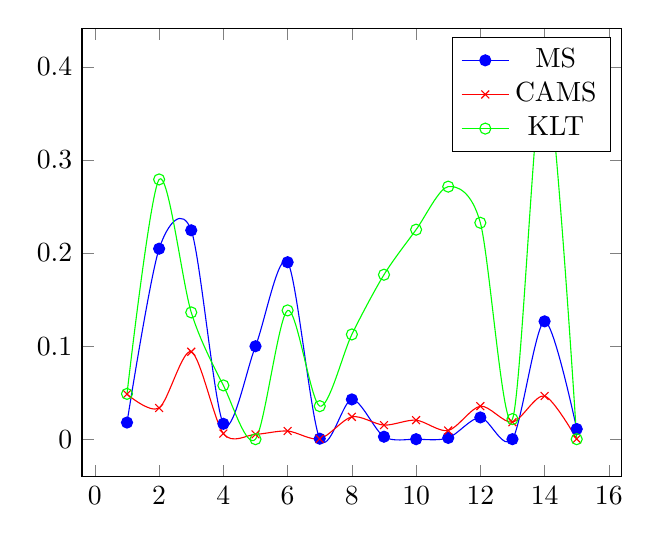
\begin{tikzpicture}
\label{figura2}
\begin{axis}
\addplot[smooth,mark=*,blue]
coordinates{
(1,0.017868877787106992)
(2,0.20464166745283086)
(3,0.22439947525641354)
(4,0.016505083791994116)
(5,0.099859793584633982)
(6,0.1901238237004759)
(7,0.00051611056428611194)
(8,0.042727525919647236)
(9,0.0026490253174241774)
(10,0.0)
(11,0.0013612595837281677)
(12,0.023374945339209762)
(13,0.0)
(14,0.12659454841132223)
(15,0.010924003231906974)
};
\addlegendentry{MS}
\addplot[smooth,color=red,mark=x]
coordinates{
(1,0.04834071999572289)
(2,0.033533440492696666)
(3,0.093966703525928355)
(4,0.0060377125773232983)
(5,0.005193923207979797)
(6,0.0087698955142402266)
(7,0.00037596389411216494)
(8,0.024013642802500183)
(9,0.015121985308645959)
(10,0.020418527632106147)
(11,0.0093192832530630734)
(12,0.035467315820262267)
(13,0.018246176158849603)
(14,0.046426220629364294)
(15,0.00020932749656048277)
};
\addlegendentry{CAMS}
\addplot[smooth,color=green,mark=o]
coordinates{
(1,0.048682322332621514)
(2,0.279069074174562)
(3,0.13620796357320028)
(4,0.057772637930407995)
(5,0.0)
(6,0.13834897983806818)
(7,0.03549622940056314)
(8,0.11253166528744955)
(9,0.17669007018779948)
(10,0.2250952493848905)
(11,0.2713289912518628)
(12,0.2325098760543383)
(13,0.02160098085837417)
(14,0.4013802649180197)
(15,0.0)
};
\addlegendentry{KLT}
\end{axis}
\end{tikzpicture}
\caption{Score by video}
\end{figure}


\begin{table}[h]
\centering
\caption{Hits}
\label{tabela2}
\begin{tabular}{|l|l|l|l|l}
\cline{1-4}
Index & MS   & CAMS & KLT  &  \\ \cline{1-4}
1     & 597  & 689  & 156  &  \\ \cline{1-4}
2     & 686  & 1071 & 266  &  \\ \cline{1-4}
3     & 575  & 534  & 1174 &  \\ \cline{1-4}
4     & 176  & 1338 & 702  &  \\ \cline{1-4}
5     & 563  & 1106 & 0    &  \\ \cline{1-4}
6     & 1191 & 1185 & 1097 &  \\ \cline{1-4}
7     & 14   & 15   & 217  &  \\ \cline{1-4}
8     & 687  & 818  & 127  &  \\ \cline{1-4}
9     & 35   & 1152 & 239  &  \\ \cline{1-4}
10    & 0    & 1794 & 264  &  \\ \cline{1-4}
11    & 7    & 1165 & 99   &  \\ \cline{1-4}
12    & 40   & 1787 & 1360 &  \\ \cline{1-4}
13    & 0    & 1788 & 3    &  \\ \cline{1-4}
14    & 136  & 826  & 829  &  \\ \cline{1-4}
15    & 116  & 181  & 0    &  \\ \cline{1-4}
\end{tabular}
\end{table}



\begin{figure}
\centering
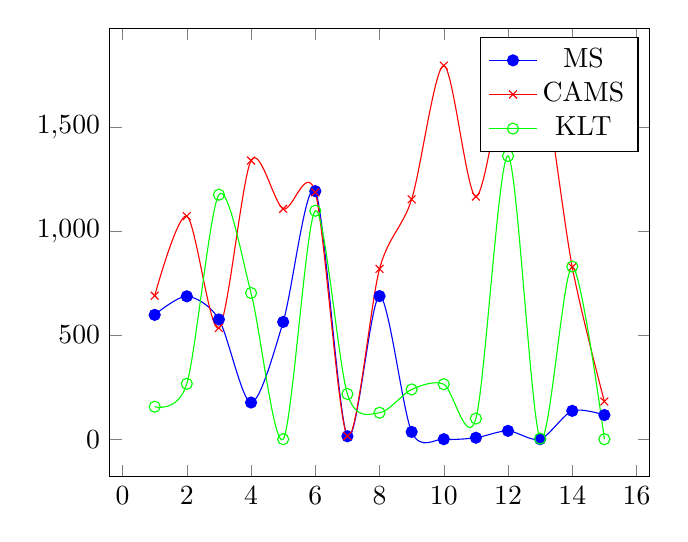
\begin{tikzpicture}
\begin{axis}
\addplot[smooth,mark=*,blue]
coordinates{
(1,597)
(2,686)
(3,575)
(4,176)
(5,563)
(6,1191)
(7,14)
(8,687)
(9,35)
(10,0)
(11,7)
(12,40)
(13,0)
(14,136)
(15,116)
};
\addlegendentry{MS}
\addplot[smooth,color=red,mark=x]
coordinates{
(1,689)
(2,1071)
(3,534)
(4,1338)
(5,1106)
(6,1185)
(7,15)
(8,818)
(9,1152)
(10,1794)
(11,1165)
(12,1787)
(13,1788)
(14,826)
(15,181)
};
\addlegendentry{CAMS}
\addplot[smooth,color=green,mark=o]
coordinates{
(1,156)
(2,266)
(3,1174)
(4,702)
(5,0)
(6,1097)
(7,217)
(8,127)
(9,239)
(10,264)
(11,99)
(12,1360)
(13,3)
(14,829)
(15,0)
};
\addlegendentry{KLT}
\end{axis}
\end{tikzpicture}
\caption{Hits by video}
\end{figure}

In the results it is possible to notice that the algorithm with more hits is not the one with the better score. The KLT algorithm often had less hits, but a better score. That happens because the polygon created by it is often smaller than the rectangles created by the others. 

Another interesting observation is that CAMeanShift will often hits every single frame. It happens because the algorithm sometimes grew the rectangle to have the same bounds as the frame. This resulted in very low scores, but high hits.

Meanshift and Camshift many times confused the skin in the hand with the skin in the arms and face. Based on our understanding of the algorithms, that was expected to happen. We found that reducing the size of the region of interest would sometimes prevent this from happening. Additionally, when there was little contrast between the hand and the background, both algorithms would loose their region of interest and select portions of the background. In videos like this, Meanshift outperformed Camshift, because it would not grow the region of interest to the whole frame.

The KLT algorithm had a few problems too. Sometimes the good features to track implementation would not find interesting points, so we had to test multiple ROI parameters for it to work in each video. We feel that a less automatic approach would bring better resuts. For example, let the user choose the points of interest in the first frame, and let KLT track them for the rest of the video.

\section{Conclusion and future work}

We have evaluated different tracking algorithms with static and moving videos of single hands performing different gestures.
Each algorithm performed best under different circumstances, and the results were compared using metrics we created.

We believe our work can be further improved by using image filters that would better isolate the hands in image. Also, machine learning algorithms could be used to find the hand in the first frame, instead of the user providing a region of interest.

\bibliographystyle{plain}
%\bibliographystyle{plainnat}
\bibliography{mylib}

\citation{Wang2009}
\citation{Kolsch2004}
\citation{Min1997}
\citation{Maggio2005}
\citation{Yin2011}
\citation{Shan2004}
\citation{Shan2007}
\citation{Ning2012}

\end{document}